\chapter{Postproduktion}

In diesem Kapitel wird der Teil der Postproduktion beschrieben. Im Zusammenhang mit diesem Projekt ist dies das Zusammenführen von Filmmaterial und gerendertem Material im Schnitt, sowie das Nachbearbeiten dieser. Die Postproduktion ist in der Videoschnitt- und Farbkorrektursoftware DaVinci Resolve 16 geschehen.

\section{Schnitt}

Der erste Schnitt wurde vor der Produktion im Zusammenhang mit dem Animatic (siehe \autoref{sec:konzept:outline}) erstellt. Aufbauend hierauf wurde auch der spätere Schnitt erstellt, dessen Übersicht in \autoref{resolve2} dargestellt ist.

\begin{figure}[H]
\begin{center}
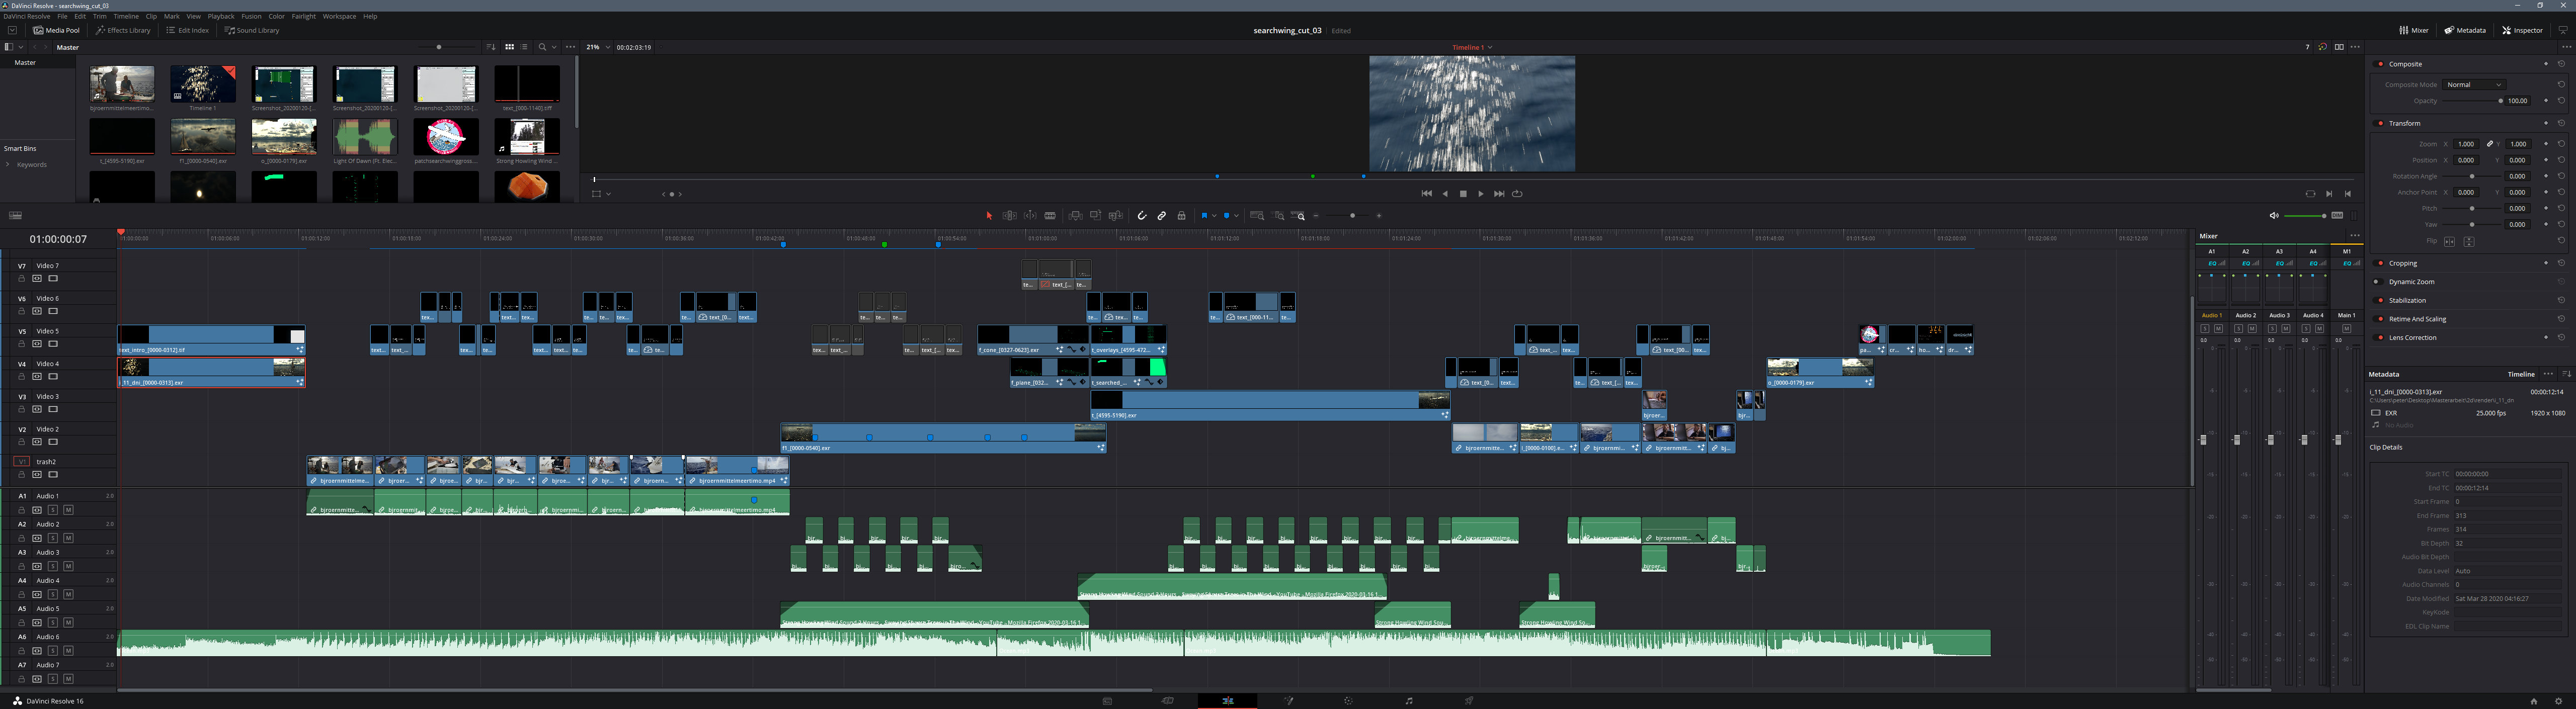
\includegraphics[width=\textwidth]{gfx/post/resolve2.jpg}
\caption{Screenshot DaVinci Resolve}
\label{resolve2}
\end{center}
\end{figure}

\section{Bauchbinden}
\label{sec:bauchbinden}

Die Texte für die Bauchbinden wurden in Blender erstellt. Der Grund ist, dass das gleichzeitige verschwinden von zwei Texten über unabhängige Masken konnte hier einfacher realisiert werden. Eine schräge Darstellung der Masken ist in \autoref{out2} abgebildet. Hierfür wurde eine Vorlage programmiert, welche für jeden neuen Text wiederholt wurde (siehe \autoref{out}).\\
Zwar wird hier wieder in Blender eine Bildsequenz erstellt, welche in das Schnittprogramm geladen wird -- trotzdem wird dieser Teil zur Nachbearbeitung des eigentlichen Filmmaterials gezählt.

\begin{figure}[H]
\begin{center}
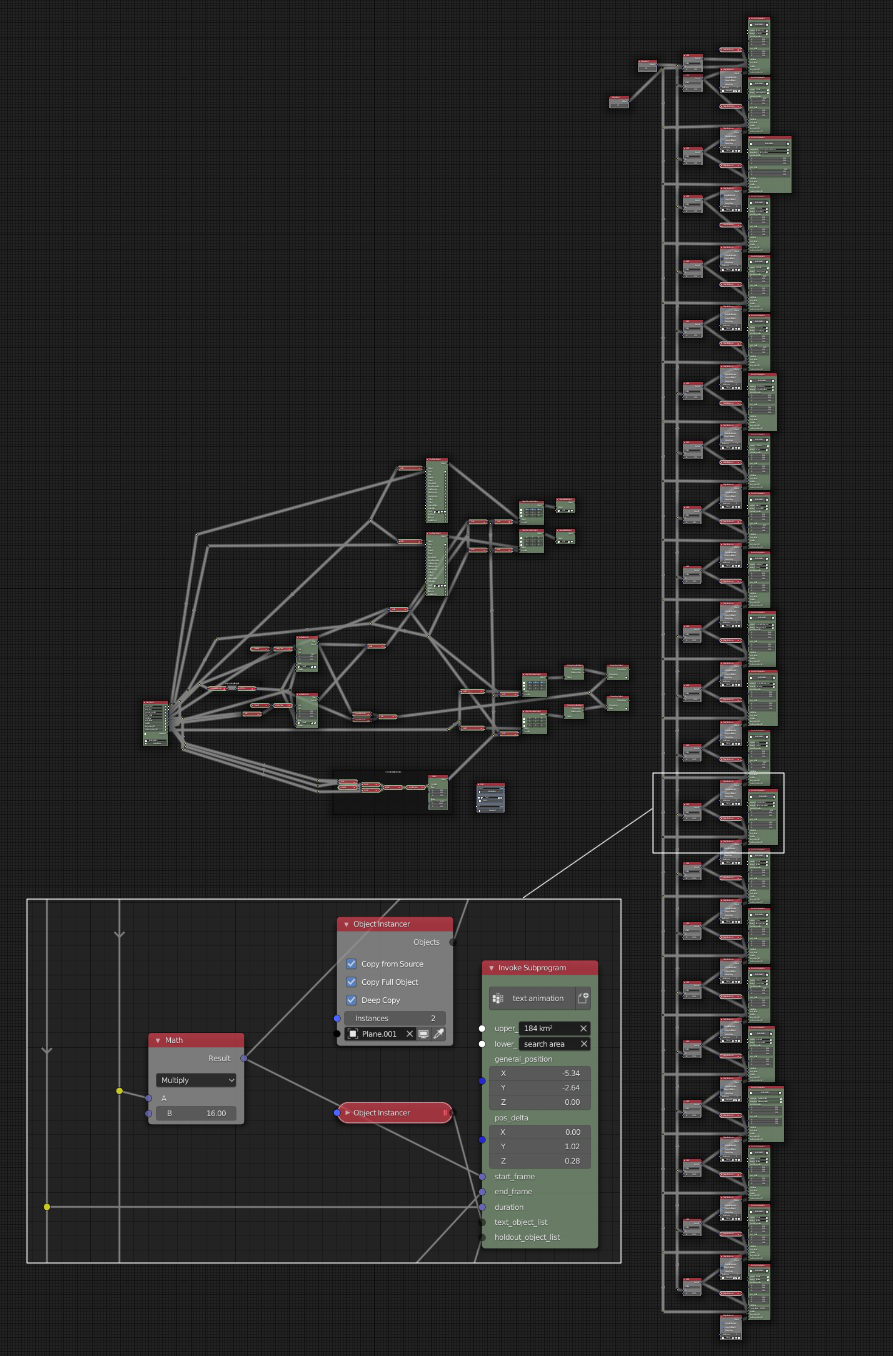
\includegraphics[width=\textwidth]{gfx/post/call-out.jpg}
\caption{Programmierte Vorlagen für die Bauchbinden}
\label{out}
\end{center}
\end{figure}

\begin{figure}[H]
\begin{center}
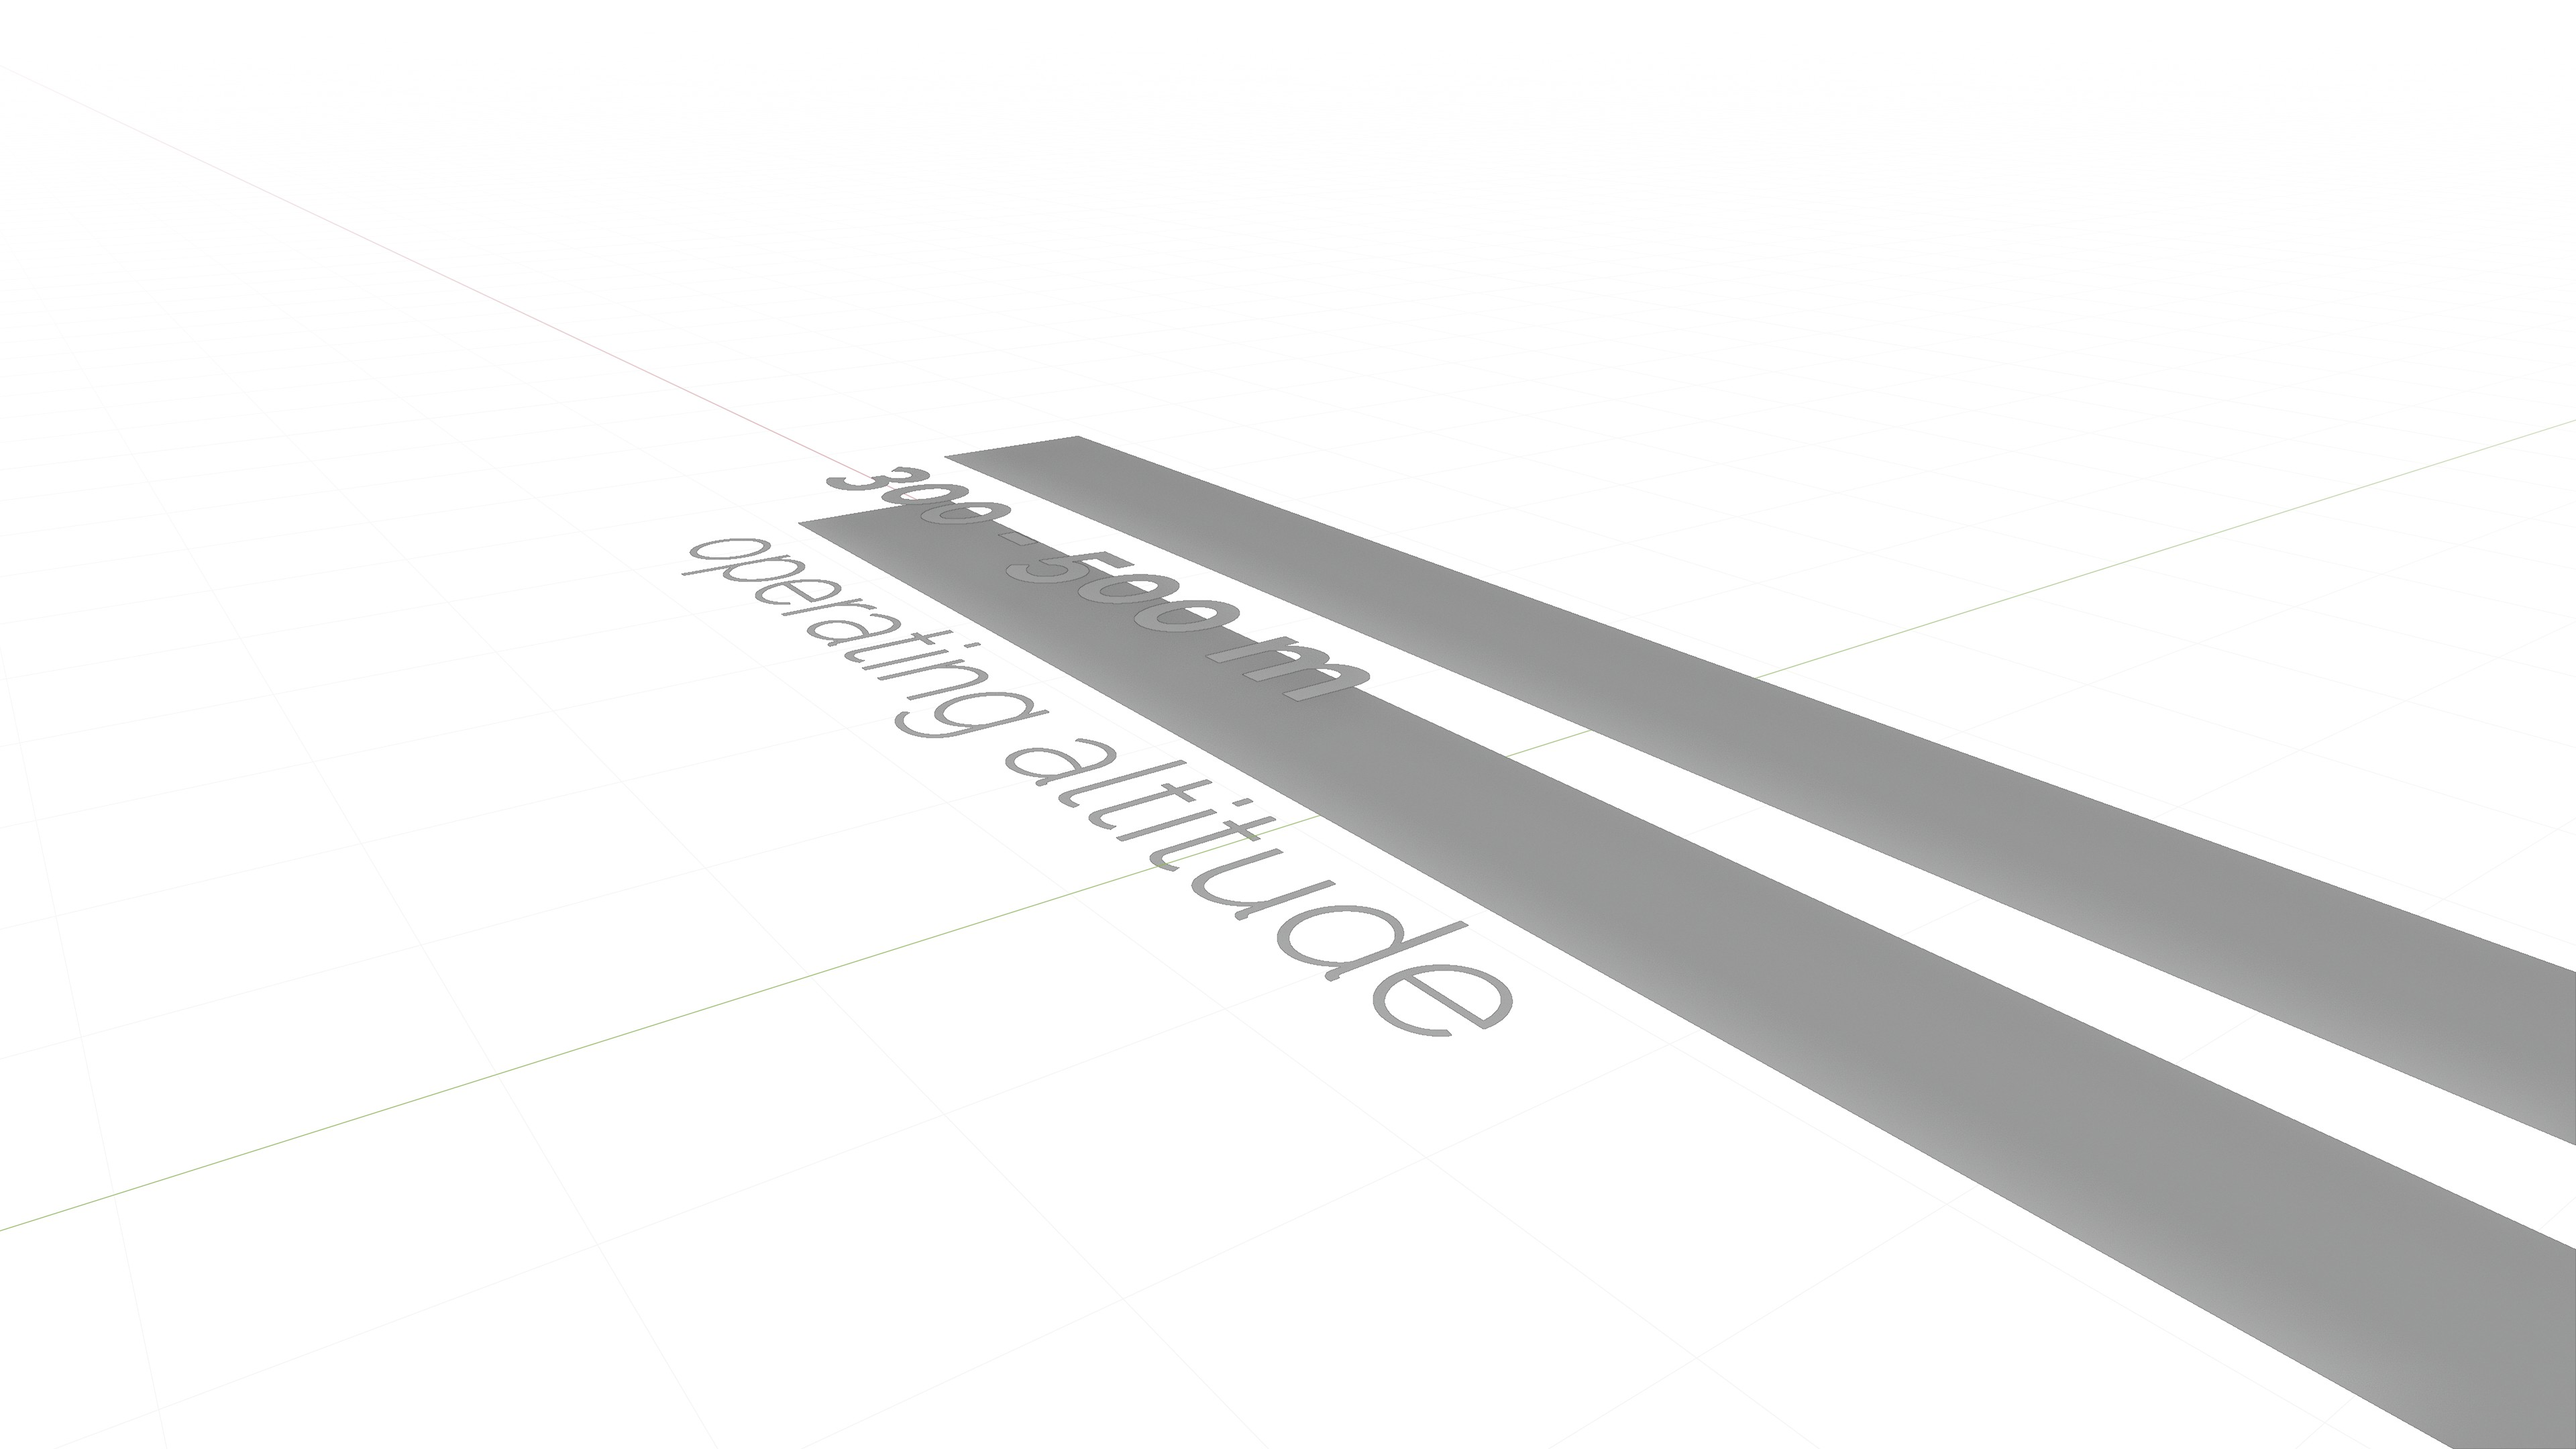
\includegraphics[width=\textwidth]{gfx/post/call-out2.jpg}
\caption{Schräge Ansicht der Masken für die Bauchbinden}
\label{out2}
\end{center}
\end{figure}

Damit der Text der Bauchbinden besser lesbar ist, wurden diese mit einem Rechteck hinterlegt, welches die Optik von satiniertem Glas hat. Dies wurde mit einem Unschärfe-Filter mit einer rechteckigen Maske realisiert. Dieser Filter musste auf alle Ebenen angewendet werden, sodass separat gerenderte Filmteile ebenfalls vom Filter betroffen werden.

\begin{figure}[H]
\begin{center}
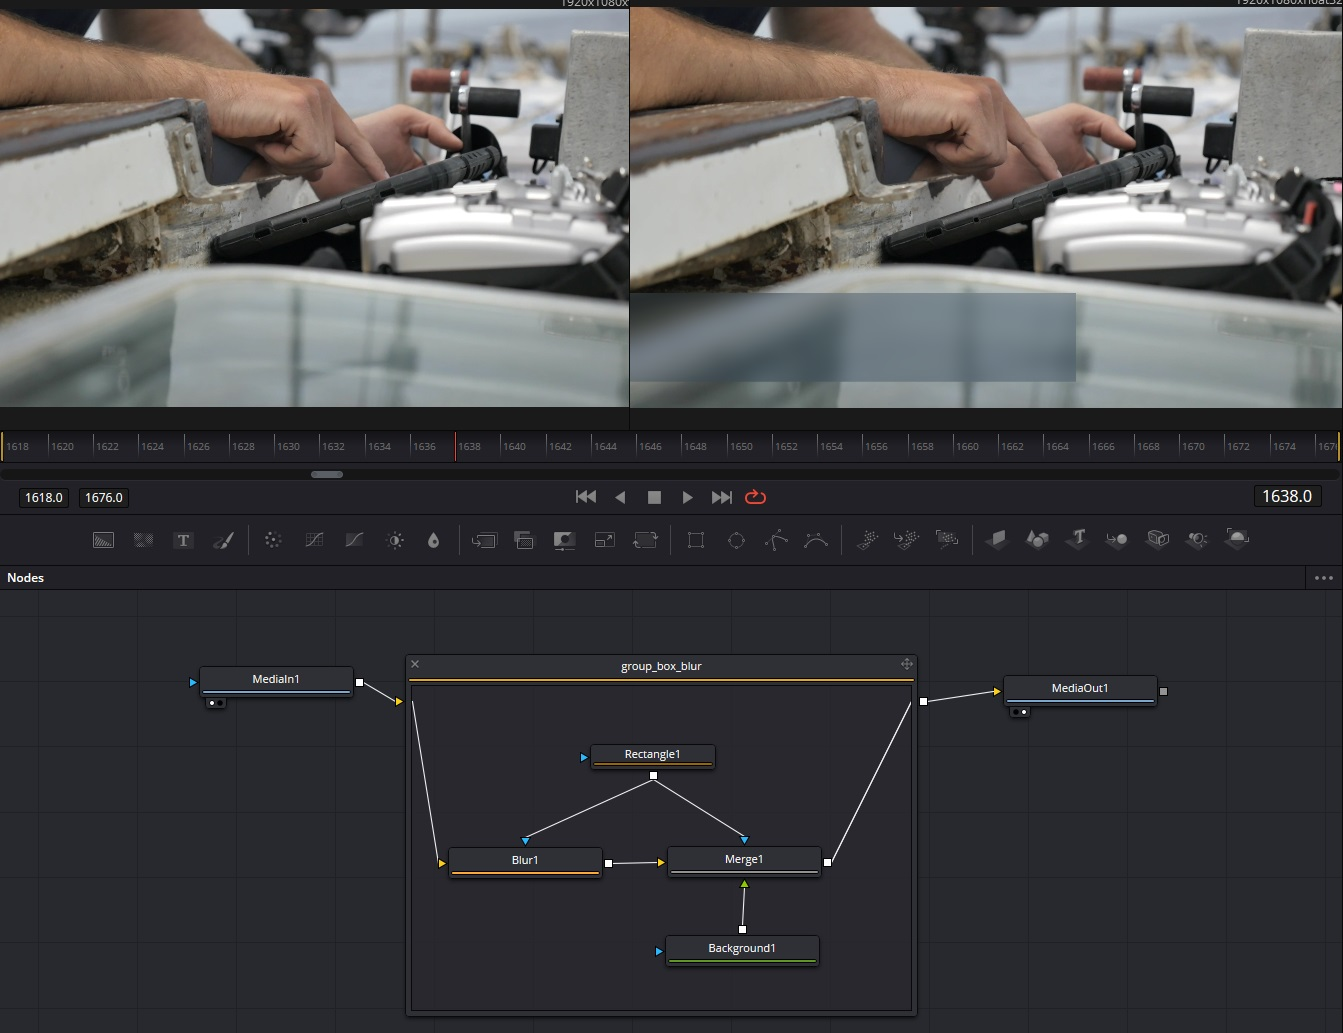
\includegraphics[width=\textwidth]{gfx/post/resolve3.jpg}
\caption{Einfügen der Bauchbinden}
\label{resolve3}
\end{center}
\end{figure}

\section{Matchmoving}

\begin{figure}[H]
\begin{center}
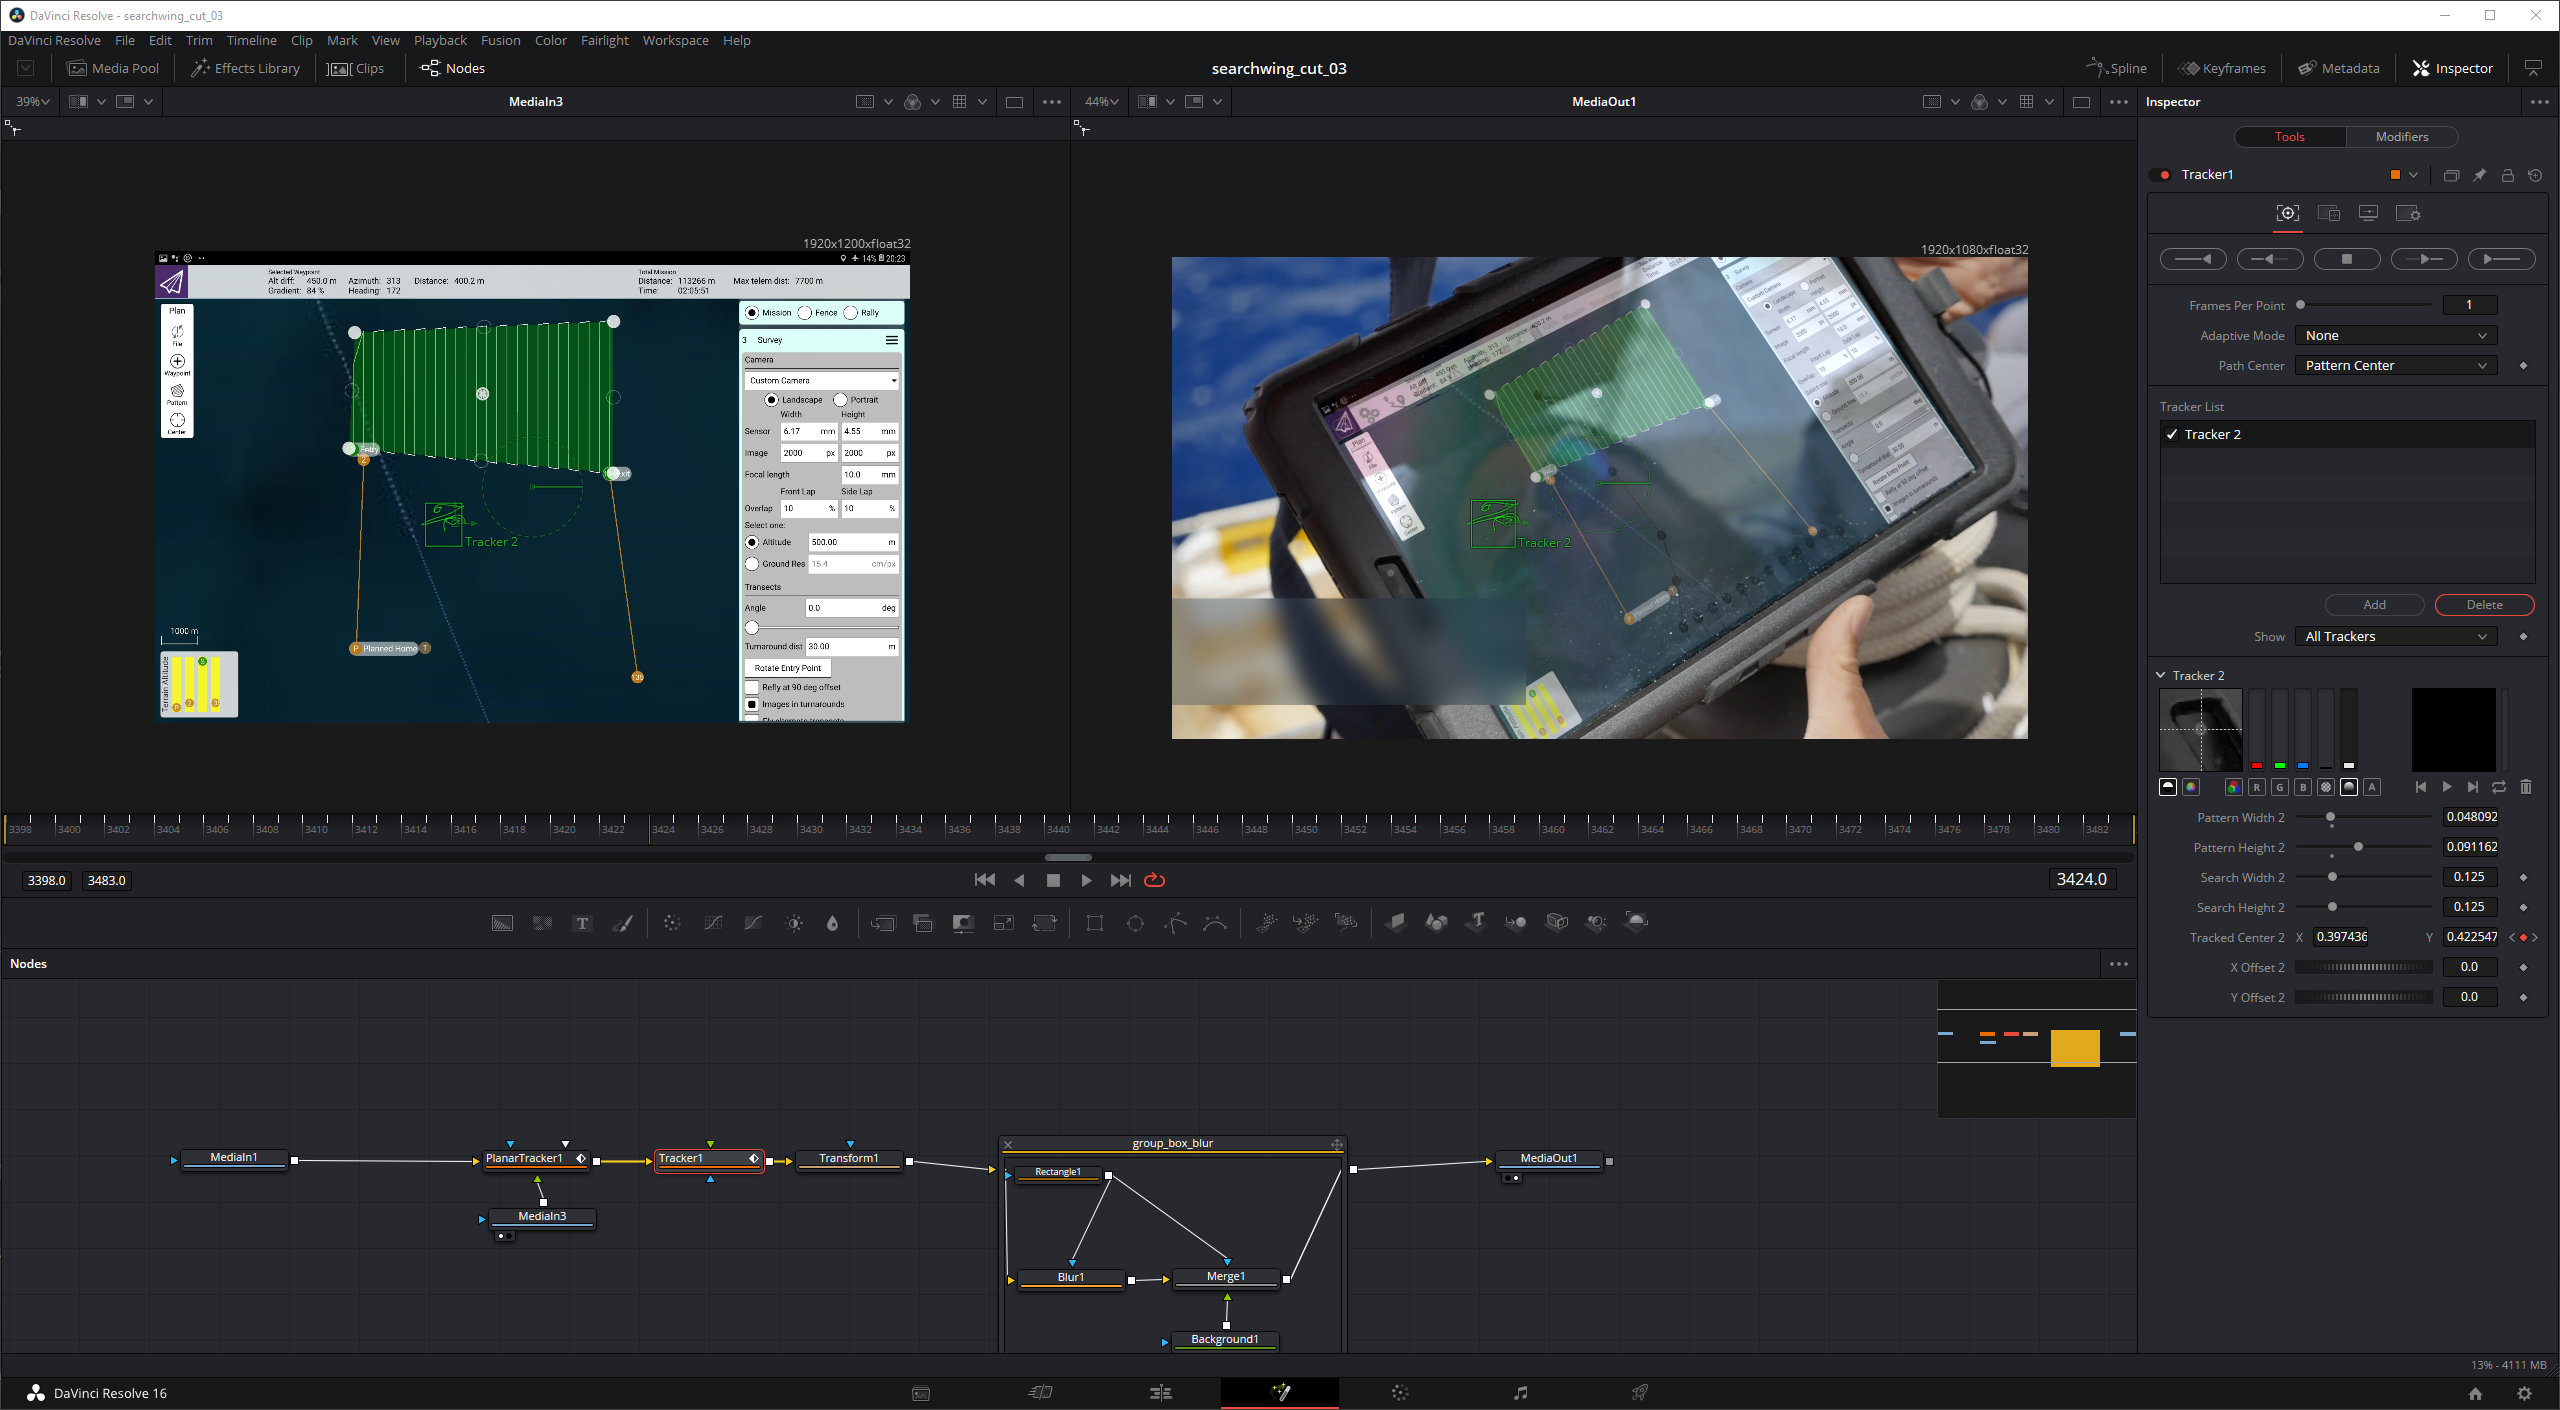
\includegraphics[width=\textwidth]{gfx/post/resolve9.jpg}
\caption{Matchmoving in der Tablet Aufnahme}
\label{resolve8}
\end{center}
\end{figure}

Das Matchmoving bezeichnet das rekonstruieren von Bewegung aus gefilmten Videomaterial. Dies wird erreicht, indem markante Punkte verfolgt werden, und anschließend aus der Bewegung dieser die Bewegung eines Objektes oder der Kamera rekonstruiert wird. \footfullcite{matchmoving}\\
In der ersten Szene, in der das Tablet sichtbar ist, wurde der Bildschirminhalt mit einem Screenshot ersetzt, da aufgrund der hellen Umgebung der Inhalt nicht gut sichtbar war. Weiterhin wurden hier mithilfe von Matchmoving ebenfalls die Bewegungen der Kamera reduziert, damit der Bildschirminhalt noch besser sichtbar ist. Ein Screenshot dieser Szene in Bearbeitung ist in \autoref{resolve8} sichtbar.\\

\begin{figure}[H]
\begin{center}
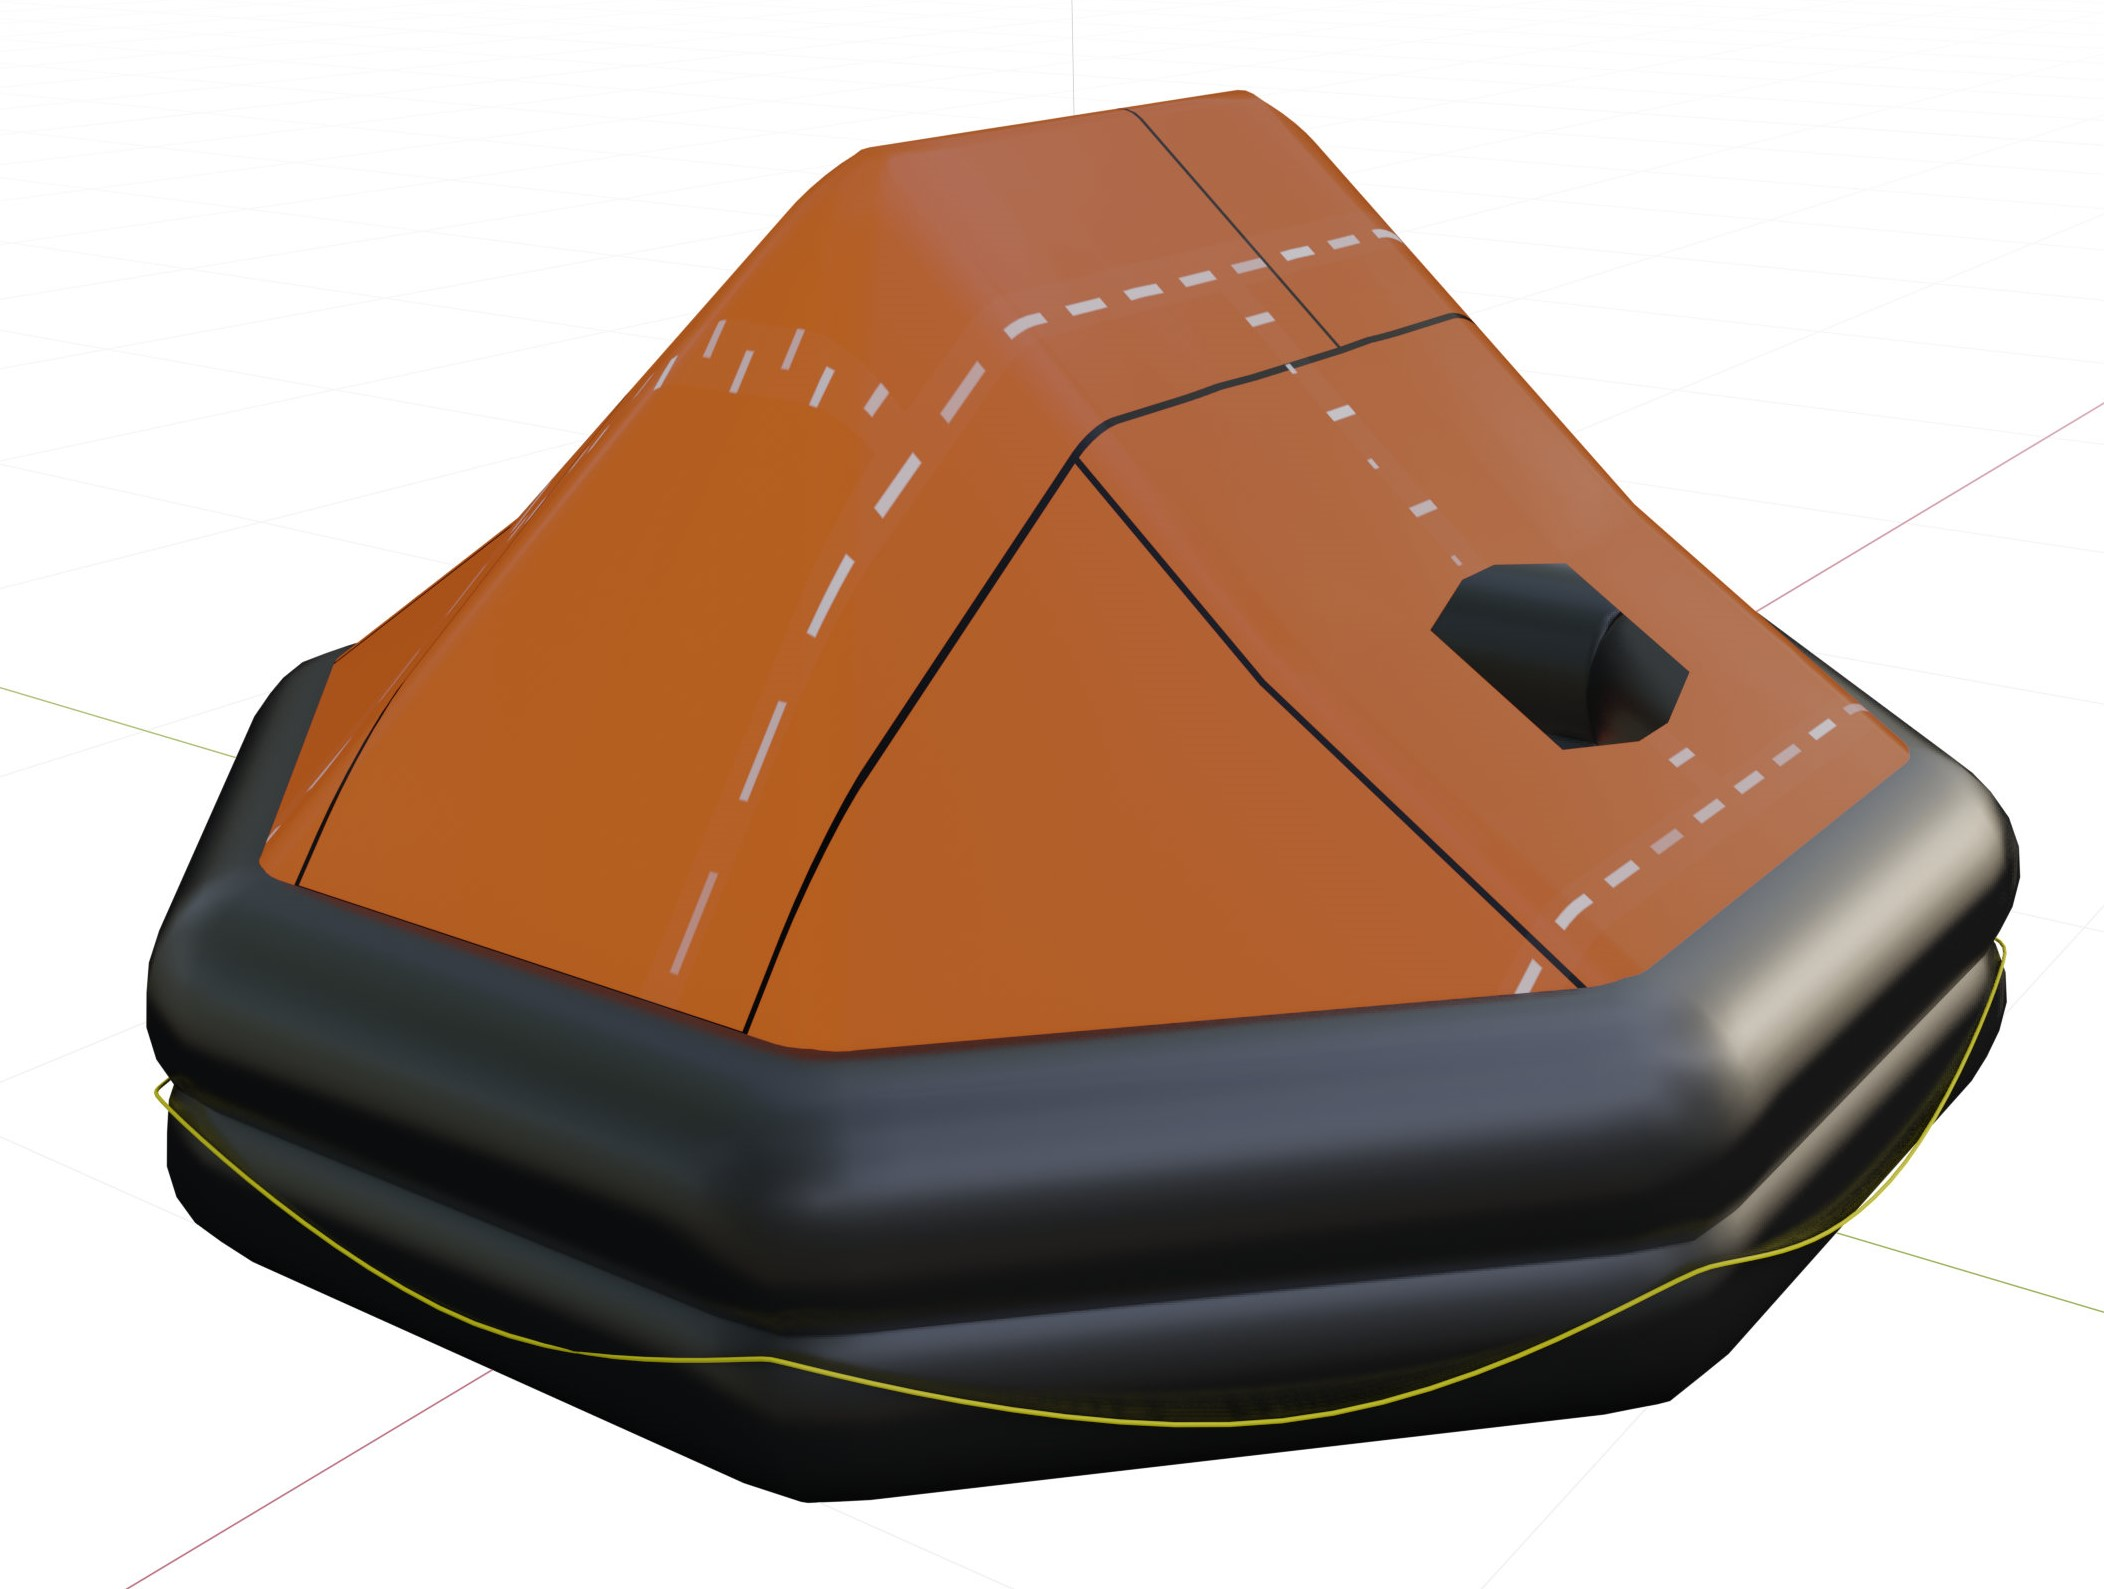
\includegraphics[width=\textwidth]{gfx/prod/boat/liferaft1.jpg}
\caption{Modell des Rettungsfloßes}
\label{liferaft1}
\end{center}
\end{figure}

Mit derselben Technik wurde ebenfalls in der Aufnahme, in der die Drohnenaufnahmen am Laptop analysiert werden, ein Rettungsfloß eingefügt. Hierzu wurde zunächst das Modell eines Rettungsfloßes erstellt (siehe \autoref{liferaft1}), dessen Bild hier eingefügt wurde (siehe \autoref{resolve10}).

\begin{figure}[H]
\begin{center}
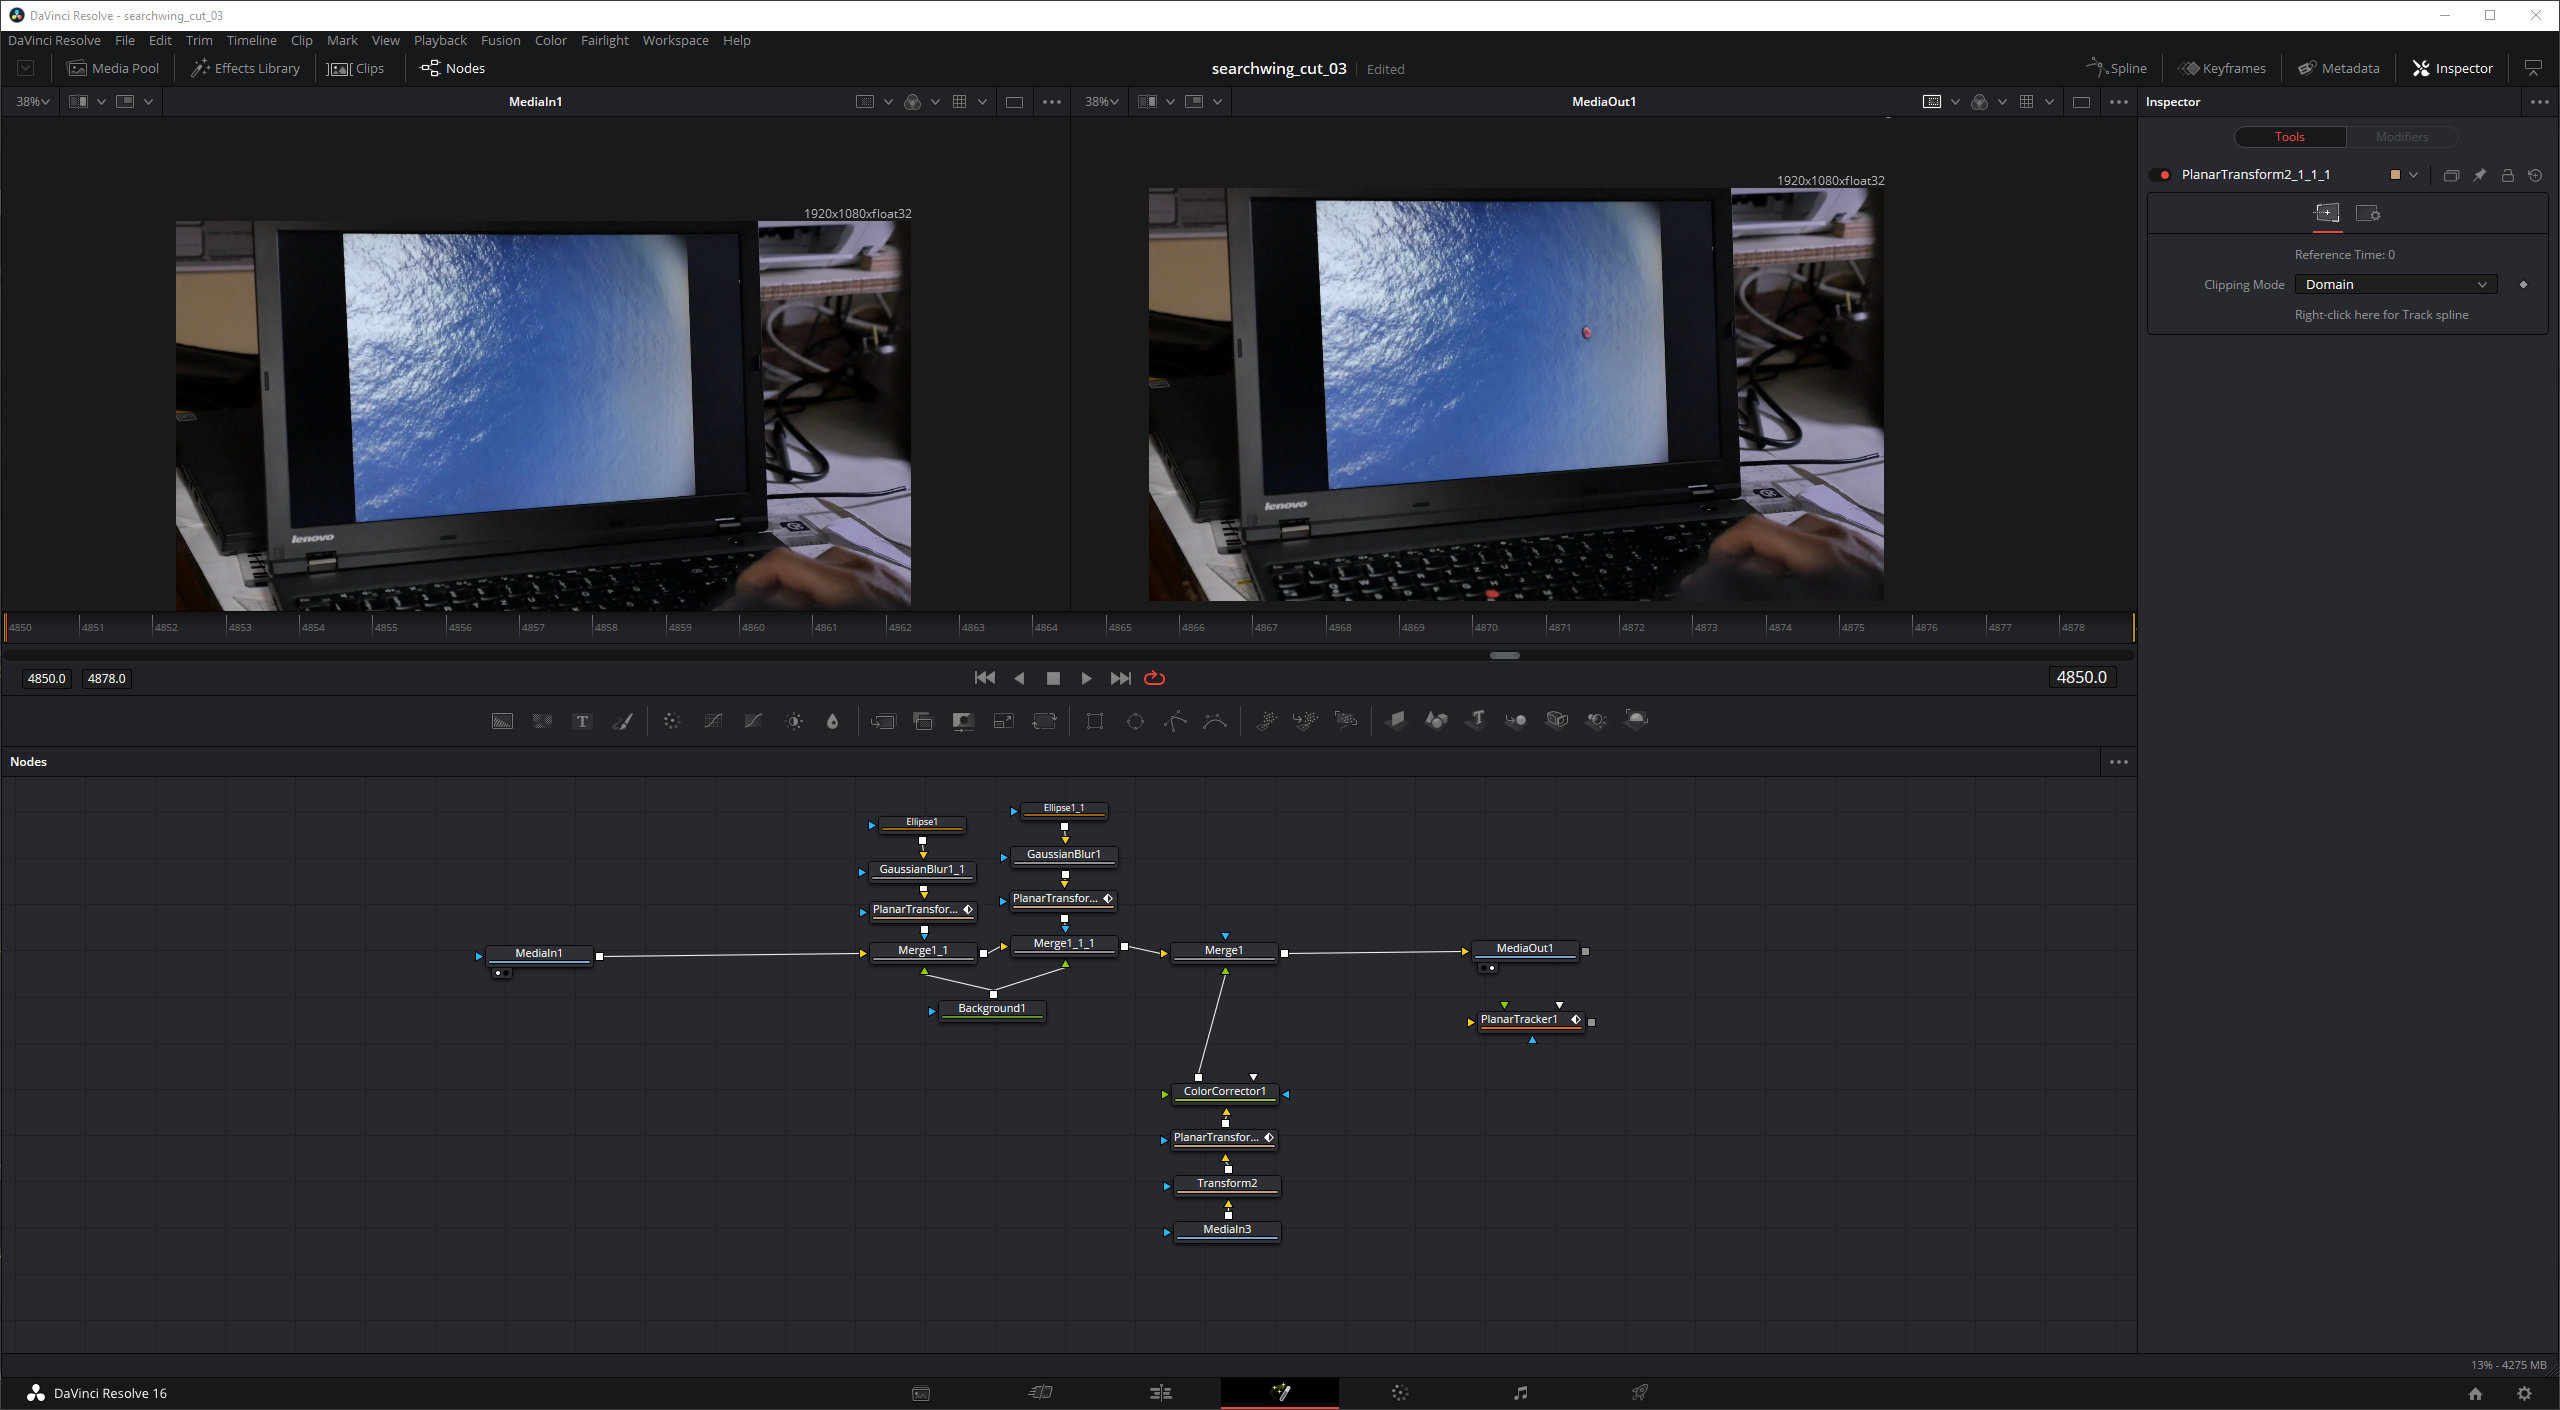
\includegraphics[width=\textwidth]{gfx/post/resolve10.jpg}
\caption{Workflow beim Einsetzen des Rettungsfloßes}
\label{resolve10}
\end{center}
\end{figure}

% \begin{figure}[H]
% \begin{center}
% 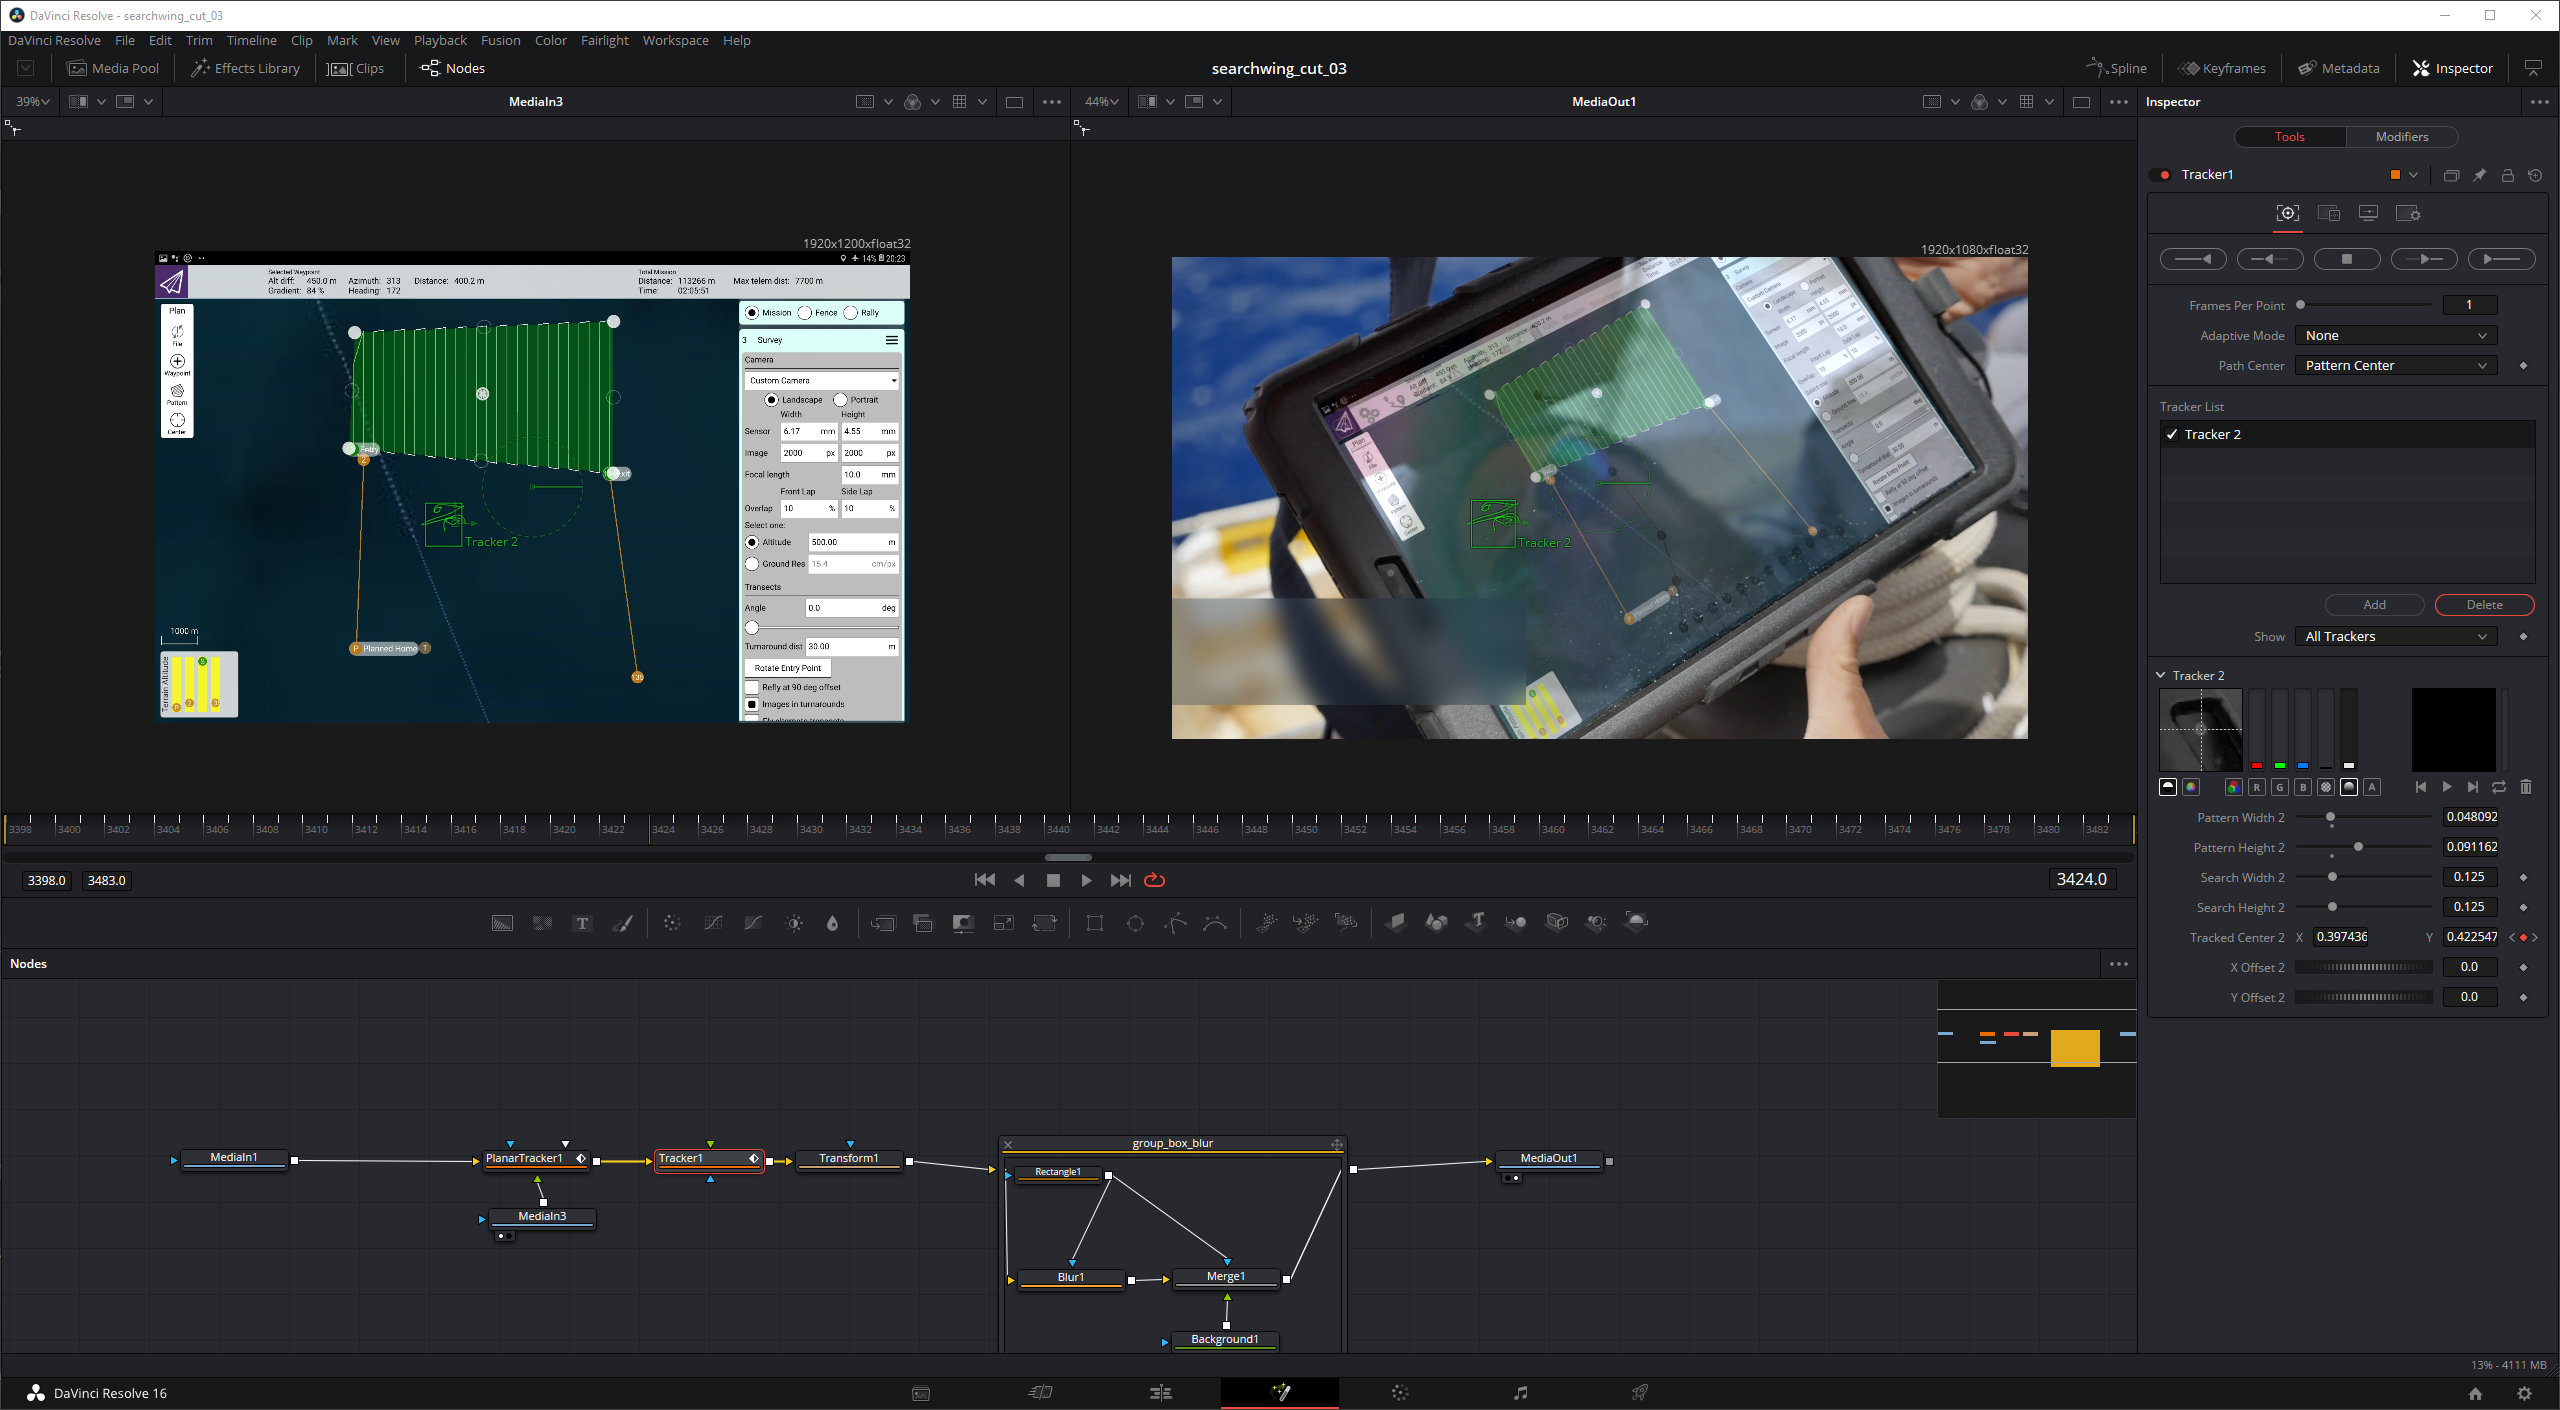
\includegraphics[width=\textwidth]{gfx/post/resolve9.jpg}
% \caption{}
% \label{resolve9}
% \end{center}
% \end{figure}

\section{Farbkorrektur}

Die gerenderten Bilder wurden weiterhin farblich an das Filmmaterial angepasst. Hierbei war sehr viel Spielraum vorhanden, da -- wie in \autoref{sec:rendering} beschrieben -- die Bildsequenz im unkomprimierten Format openEXR aus Blender exportiert wurde. Dieses Format besitzt eine sehr hohe Farbtiefe, da pro Farbkanal eine 32-Bit-Gleitkommazahl gespeichert wird. \footfullcite{openexr}\\
Weiterhin wurde beachtet, dass ein kompletter linearer Workflow vorhanden ist. Dies bedeutet, dass Bildmaterial, das miteinander kombiniert wird, im linearen Farbraum bearbeitet wird, und erst nachdem sie fertig kombiniert sind, Farbkorrekturen angewendet werden. Wird dies nicht beachtet, entstehen bspw. Stellen, an denen das Bild ausbrennt. \footfullcite{linearworkflow}\\
Nachdem die unterschiedlichen Ebenen, wie Drohne und illustrierende Überlagerungen kombiniert wurde, wurde der Farbraum aus Blender wieder angewendet. Hierbei handelt es sich um den Farbraum ``Filmic''. Dieser simuliert das Verhalten eines analogen Filmes, indem bspw. die Helligkeit nicht mehr linear, sondern logarithmisch steigt, oder helle Pixel entsättigt werden. \footfullcite{filmic}\\
Die Anpassungen der Farben ist zunächst durch den Weißpunkt geschehen. Hierdurch wurde die Helligkeit ebenfalls angepasst. Dabei wird ein Pixel des Bildes selektiert, der den hellsten Punkt des Bildes darstellt. Die Farben des Bildes werden anschließend automatisch so angepasst, dass dieser Punkt reines Weiß ist.\\
Die restlichen Farbanpassungen sind über die ``Color Wheels'' geschehen. Mithilfe dieser können die Farben in unterschiedlichen Helligkeitsbereichen angepasst werden. \footfullcite{colorcorrect}


\begin{figure}[H]
\begin{center}
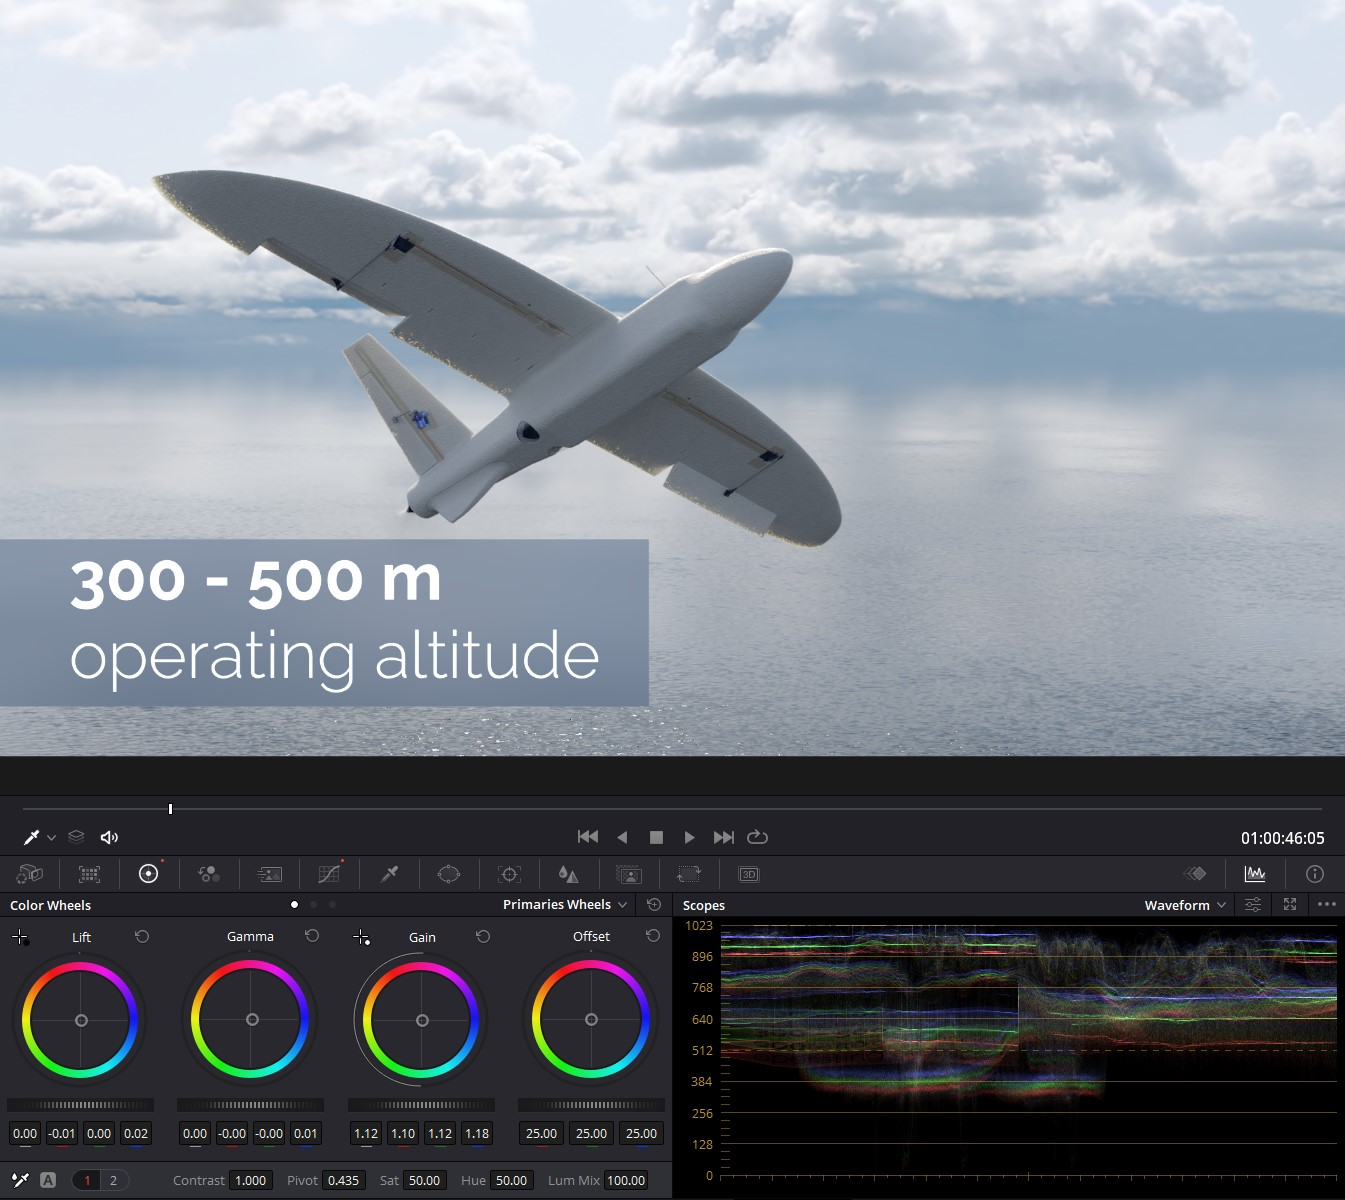
\includegraphics[width=\textwidth]{gfx/post/resolve7.jpg}
\caption{Workflow bei der Anpassung der Farben}
\label{resolve7}
\end{center}
\end{figure}

\section{Audio}

Die Entscheidung des Musiktitels fiel auf den Song Ocean von Thbd. Dieser Musiktitel wurde gewählt, da dieser sehr gut die Fluggeschwindigkeit der Drohne widerspiegelt. Zudem war der Rhythmus weder zu aufdringlich, noch fehlte die nötige Dynamik. Die Ernsthaftigkeit des Themas, aber auch die Zuversicht wurde durch diesen Musiktitel gekonnt untermalt.\\
Der Titel hat in der Originalfassung eine Länge von 3:46 und der Film von 2:04. Daher wurde der Titel in der Länge angepasst, indem bei etwa 0:56 das Lied geteilt wurde, und ein Teil aus der Mitte entfernt wurde. Diese Stelle wurde gewählt, da hier ein starker Wechsel der Bildsprache von der Seitenansicht, zur Draufsicht des Flugpfades stattgefunden hat. Außerdem waren somit das Intro, als auch das Outro des Musiktitels an der passenden Stelle.\\
Ergänzend zu der Musik wurden Soundeffekte für den Flug hinzugefügt. Hierbei wurde die Audiospur einer Videoaufnahme der Drohne als Motorsound verwendet. Dieser war vergleichsweise kurz, und musste daher mehrmals nacheinander wiedergegeben werden, wie in \autoref{sample} dargestellt ist. Um den Effekt des ständig wiederholenden Audioeffektes zu umgehen, wurden einige Instanzen der Audiospur rückwärts abgespielt. Dass der Motorsound und die Musik dieselbe Tonhöhe haben, war ein glücklicher Zufall.\\

\begin{figure}[H]
\begin{center}
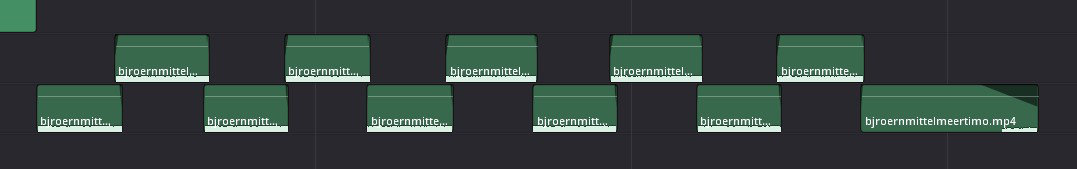
\includegraphics[width=\textwidth]{gfx/post/sample.jpg}
\caption{Wiederholung des Motorsounds der Drohne}
\label{sample}
\end{center}
\end{figure}

Abschließend wurden Windgeräusche unter den Flug der Drohne gelegt, damit das Geschwindigkeitsgefühl weiter untermalt wird. \footfullcite{wind}

\begin{figure}[H]
\begin{center}
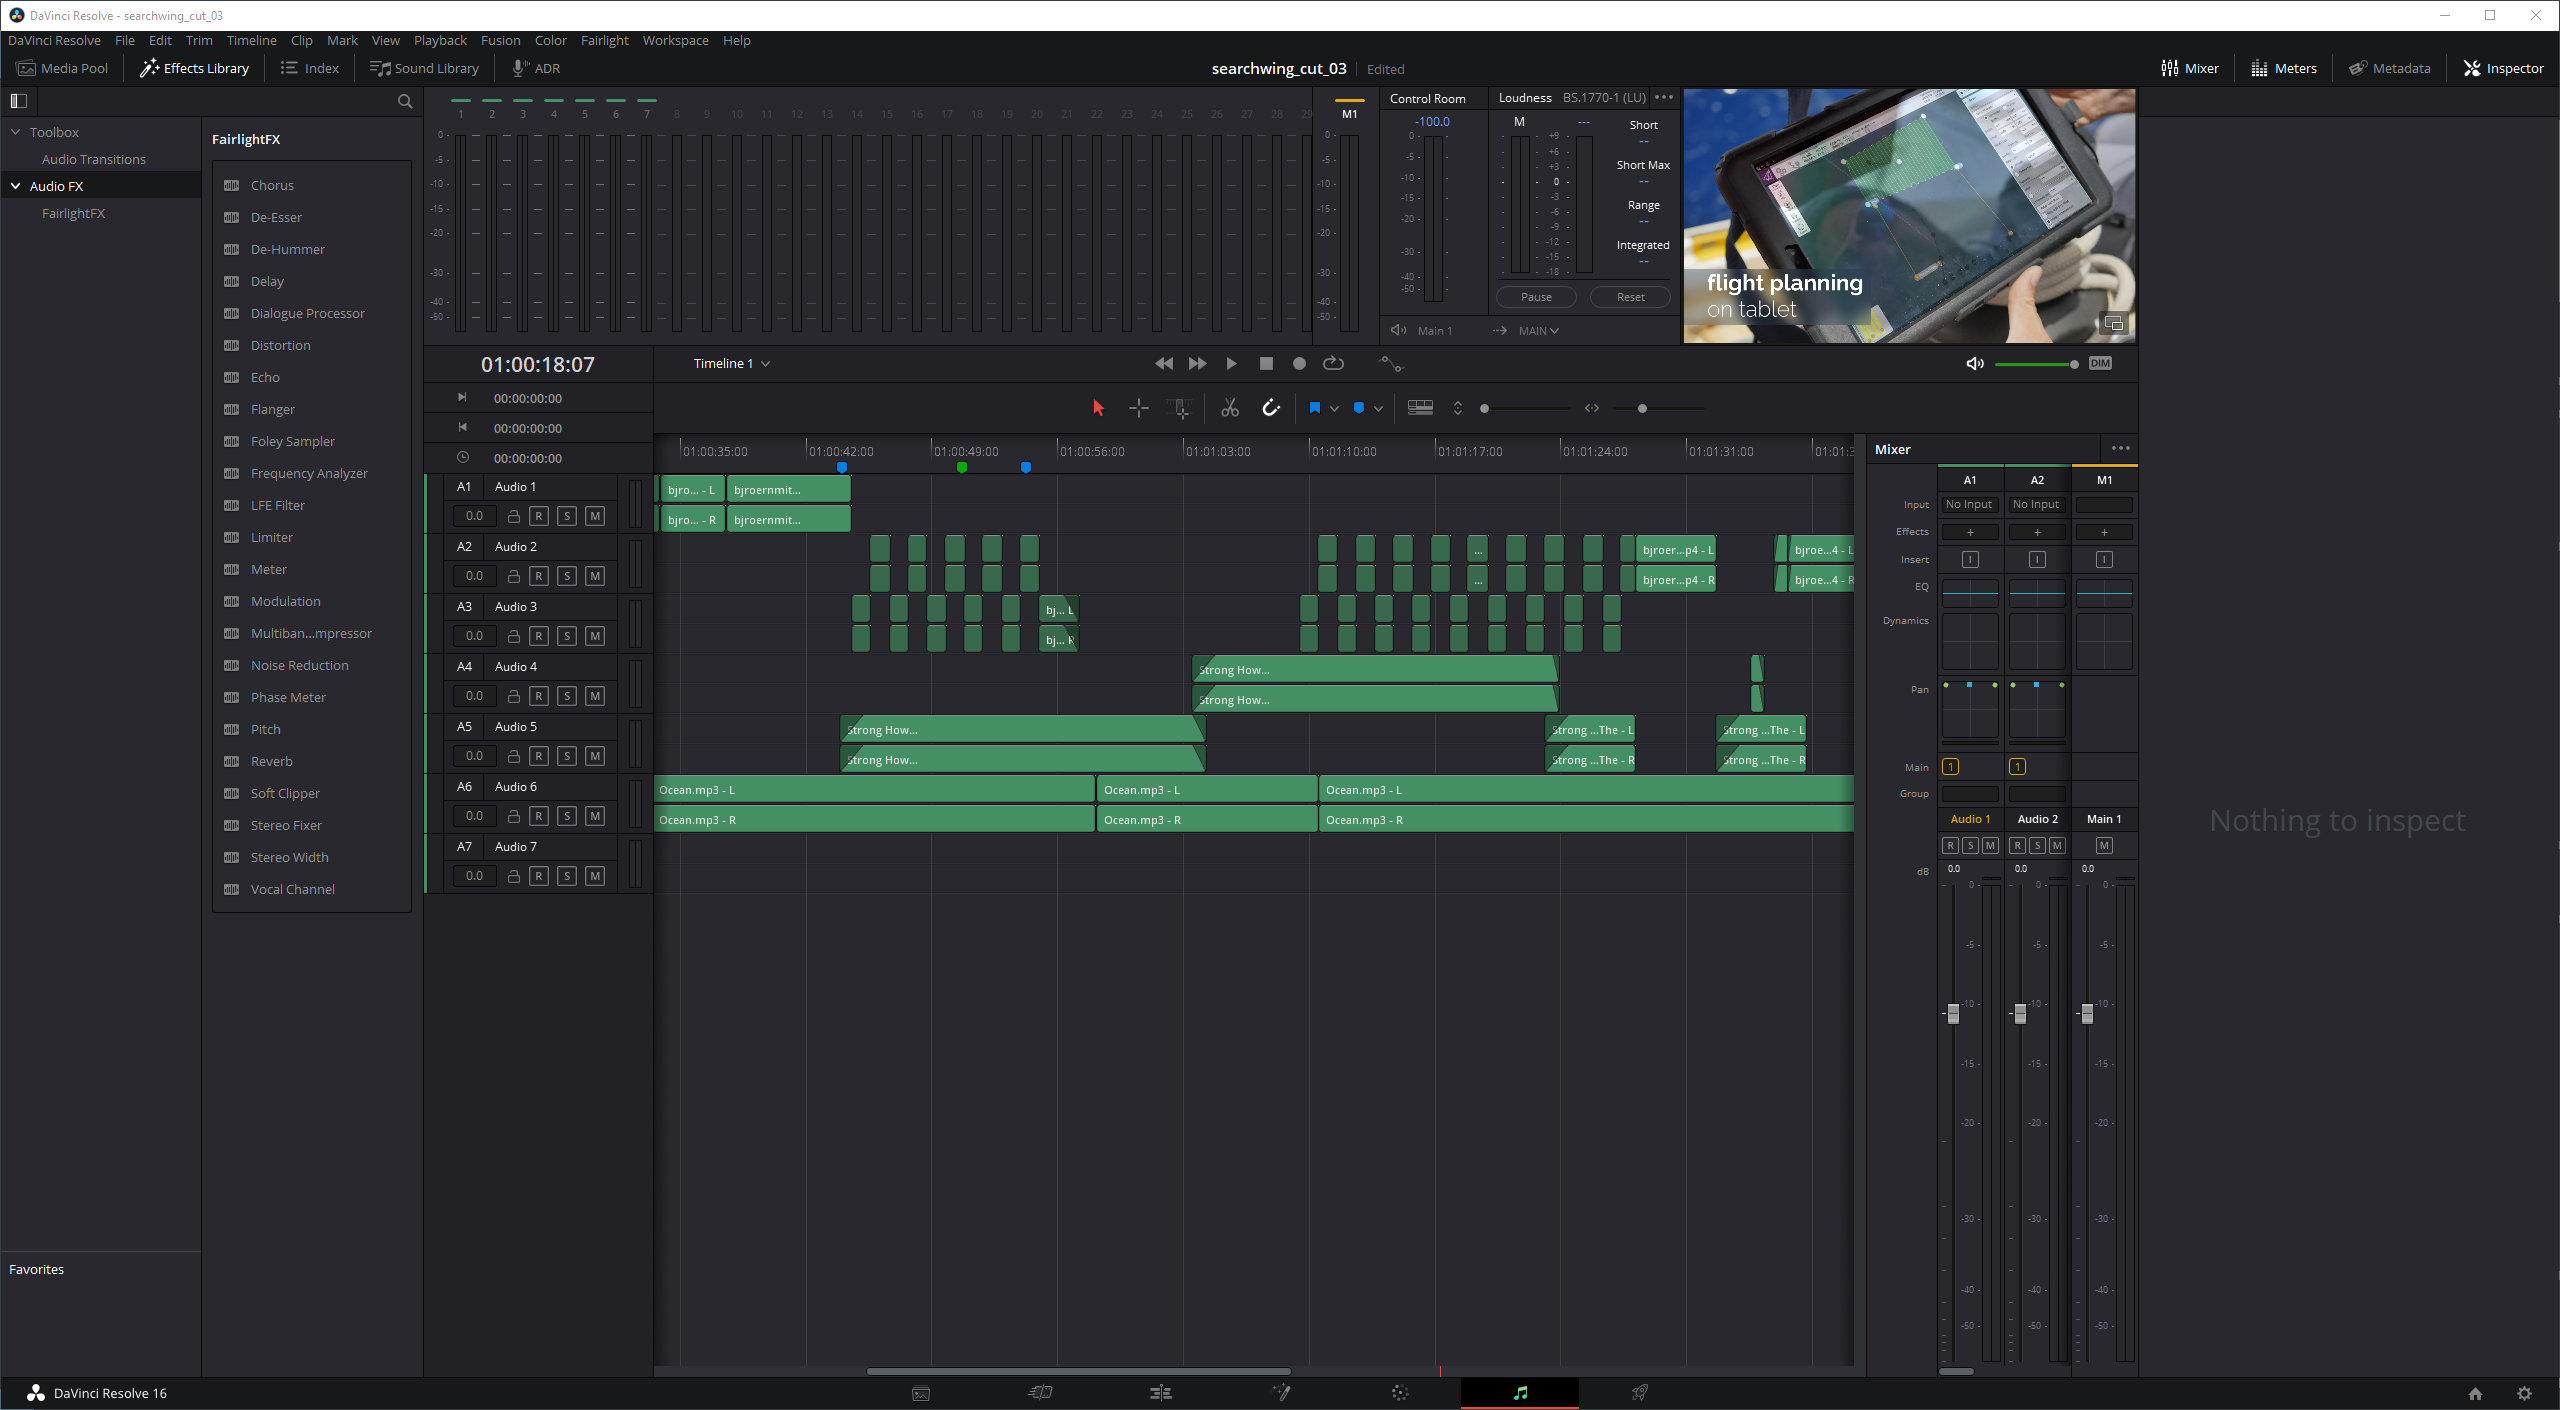
\includegraphics[width=\textwidth]{gfx/post/resolve1.jpg}
\caption{Übersicht der Audiospuren}
\label{resolve1}
\end{center}
\end{figure}
